\chapter{Datos y metodología}\label{cap:3}

\section{Datos}\label{sec:datos}

El análisis utiliza dos fuentes de precipitación diaria. Como referencia observacional se emplea CR2MET v2.5 (Centro de Ciencia del Clima y la Resiliencia, CR2), un producto grillado de precipitación diaria para Chile en una grilla regular de latitud--longitud de 0,05° (\textasciitilde5 km). CR2MET combina observaciones de estaciones con información de reanálisis y se usa de manera rutinaria como referencia hidroclimática en el país (Álvarez-Garretón et al., 2018; Latoja et al., 2025; Herrera-Marín et al., 2026). Como modelo climático regional se utiliza la simulación CNRM-ALADIN64 sobre el dominio CHP12 (\textasciitilde12 km). Su precipitación, entregada en kg m$^{-2}$ s$^{-1}$, se convierte a mm día$^{-1}$ multiplicando por 86 400. Se usa una única simulación regional, de modo que la comparación entre histórico y futuro se realiza dentro de un mismo modelo; como sensibilidad al escenario, los risk ratios se repiten con SSP3-7.0 (Anexo~\ref{sec:S6}), y la incertidumbre asociada a otros modelos se discute en §\ref{sec:limitaciones}.

El dominio de estudio es Chile continental. La máscara terrestre se construye con la geometría de Chile de Natural Earth (escala 1:10 m), considerando las celdas de ALADIN cuyo centro cae dentro del polígono, lo que resulta en 3 587 celdas. Para permitir comparaciones píxel a píxel, CR2MET se interpola linealmente a los centros de celda de la grilla de ALADIN. Esta interpolación introduce un suavizado leve de CR2MET y no conserva exactamente la precipitación integrada del dominio.

Se analizan dos ventanas de 35 años: el histórico 1980--2014 (CR2MET y ALADIN) y el futuro 2040--2074 bajo SSP5-8.5 (solo ALADIN). El histórico termina en 2014, año final del experimento histórico de CMIP6, de modo que no mezcla forzante histórico y de escenario; el futuro representa mediados de siglo. Al tener ambas ventanas la misma longitud, el tamaño muestral no condiciona la comparación histórico--futuro.

Las PDFs de duración se calculan en cuatro ventanas representativas del gradiente climático chileno: Loa (norte árido), Maipo y Maule (zona central mediterránea) y Biobío (sur más húmedo). No son polígonos oficiales de cuenca, sino cajas de latitud--longitud sobre la grilla de ALADIN, intersectadas con la máscara continental, y se eligieron como casos de estudio a lo largo del gradiente norte--sur. Los risk ratios se calculan sobre cuatro regiones administrativas completas (Coquimbo, O'Higgins, La Araucanía y Los Lagos; geometrías de Natural Earth), unidades usadas en la gestión hídrica y agrícola. Las cajas se usan para describir la forma de la PDF, en particular su cola, y las regiones para cuantificar el cambio en el número de rachas largas (Figura~\ref{fig:dominio}; Tabla~\ref{tab:datos}).

\begin{figure}[htbp]
\centering
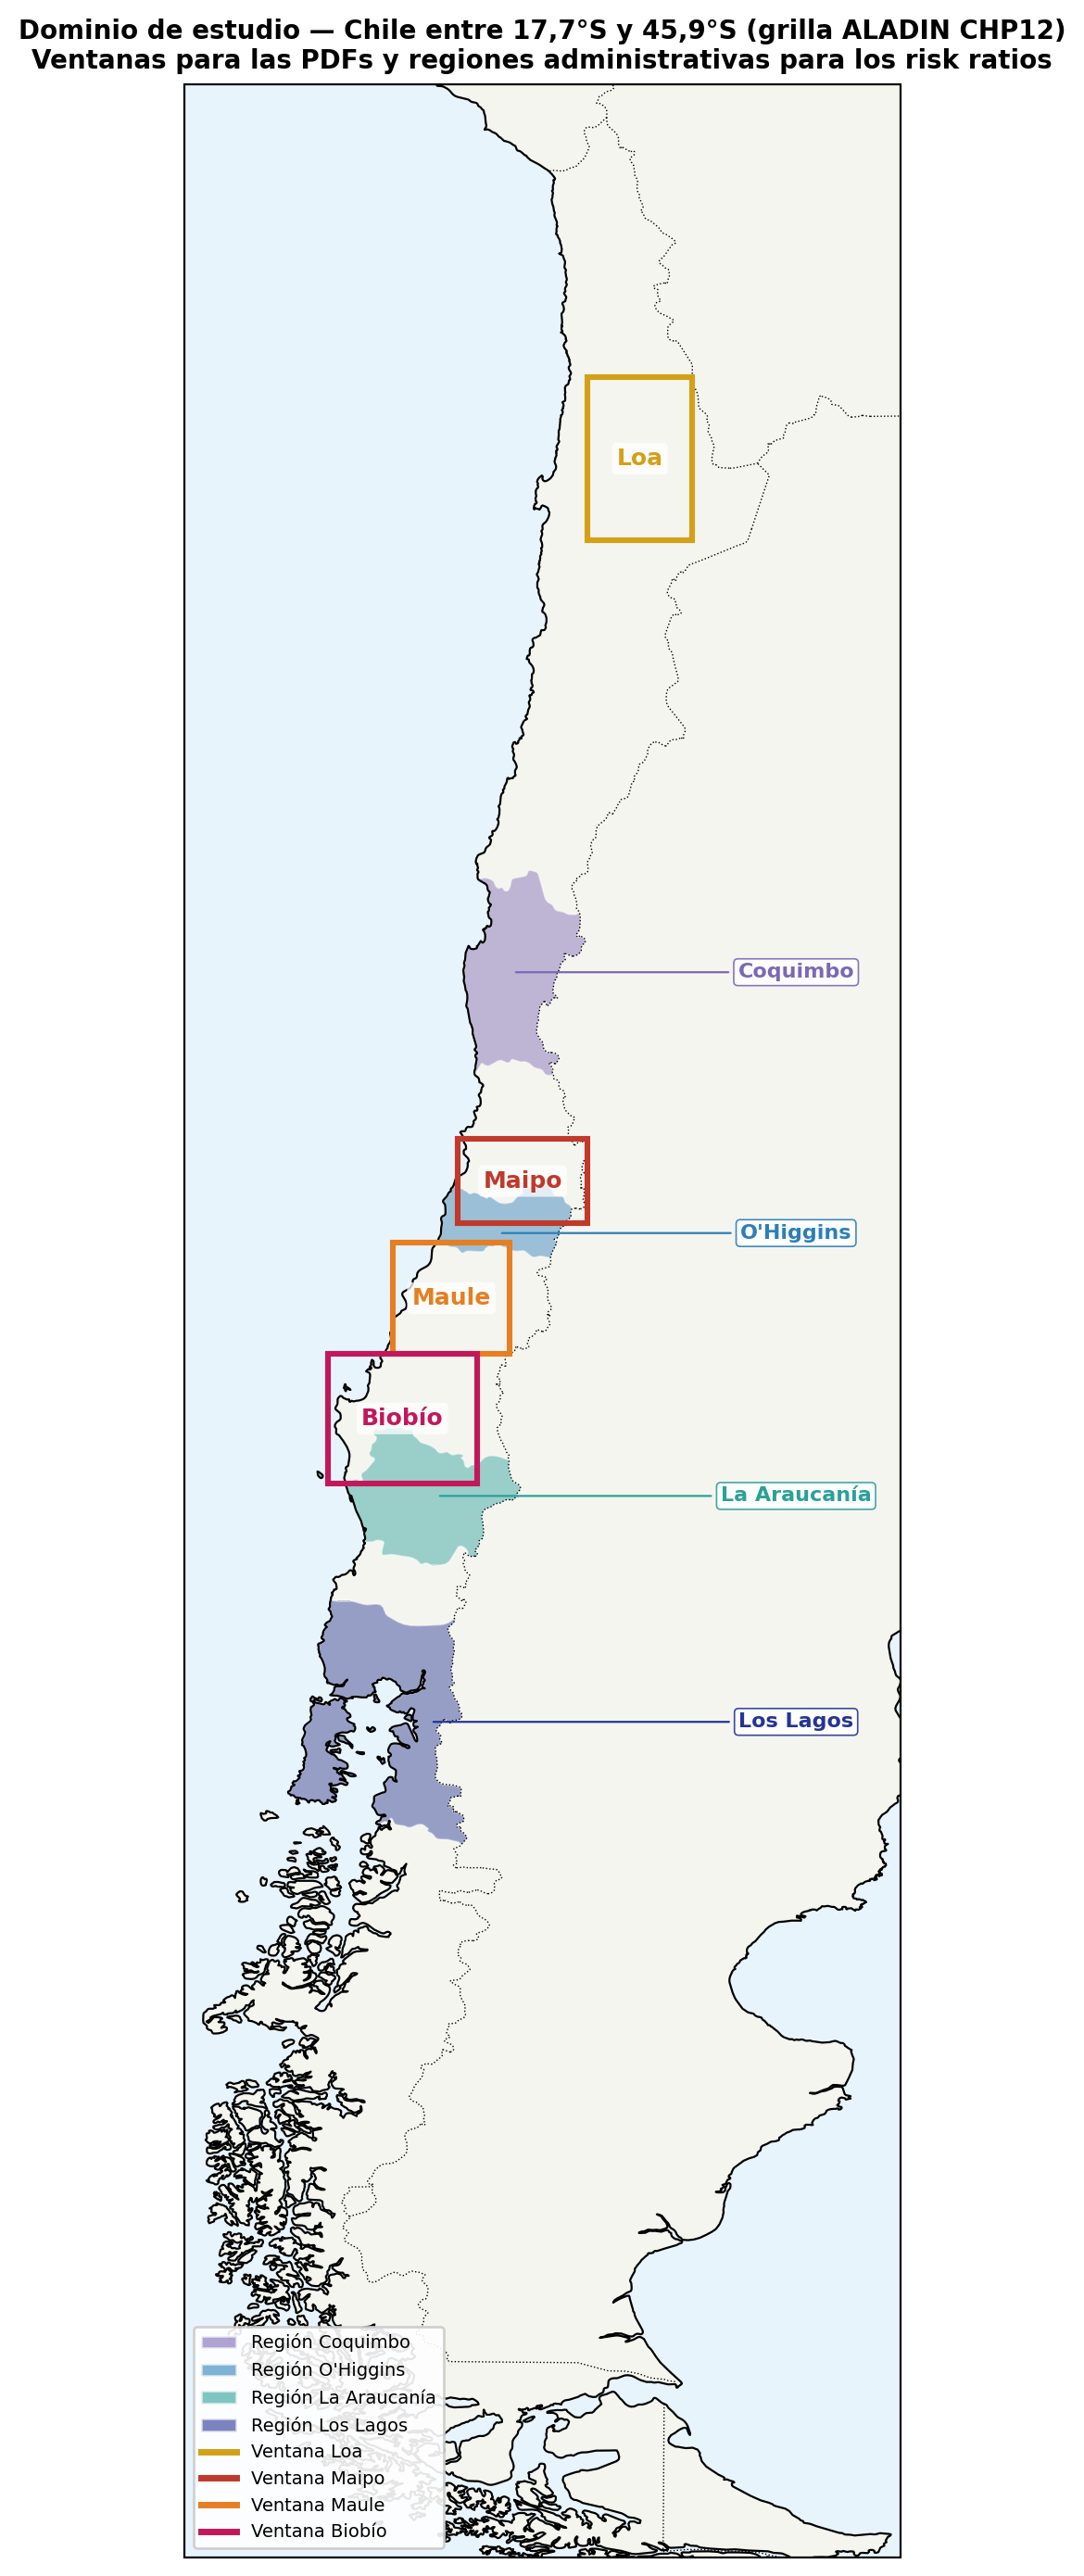
\includegraphics[width=1\linewidth,height=0.72\textheight,keepaspectratio,alt={Dominio de estudio sobre Chile continental. Los rectángulos indican las ventanas de latitud--longitud usadas para las PDFs de duración de dry spells: Loa (21,5--24,0°S; 68,2--69,8°O; 298 celdas), Maipo (33,2--34,5°S; 69,8--71,8°O; 154 celdas), Maule (34,8--36,5°S; 71,0--72,8°O; 171 celdas) y Biobío (36,5--38,5°S; 71,5--73,8°O; 243 celdas). Las ventanas aproximan las cuencas que les dan nombre sin coincidir con sus límites; en particular, la ventana Loa abarca la cuenca alta del Loa y la cuenca del Salar de Atacama, ambas representativas del norte árido. Las áreas sombreadas son las regiones administrativas usadas para los risk ratios: Coquimbo (239 celdas), O'Higgins (110), La Araucanía (223) y Los Lagos (324).}]{fig02_dominio_cuencas_regiones.png}
\caption[Dominio de estudio sobre Chile continental]{Dominio de estudio sobre Chile continental. Los rectángulos indican las ventanas de latitud--longitud usadas para las PDFs de duración de dry spells: Loa (21,5--24,0°S; 68,2--69,8°O; 298 celdas), Maipo (33,2--34,5°S; 69,8--71,8°O; 154 celdas), Maule (34,8--36,5°S; 71,0--72,8°O; 171 celdas) y Biobío (36,5--38,5°S; 71,5--73,8°O; 243 celdas). Las ventanas aproximan las cuencas que les dan nombre sin coincidir con sus límites; en particular, la ventana Loa abarca la cuenca alta del Loa y la cuenca del Salar de Atacama, ambas representativas del norte árido. Las áreas sombreadas son las regiones administrativas usadas para los risk ratios: Coquimbo (239 celdas), O'Higgins (110), La Araucanía (223) y Los Lagos (324).}\label{fig:dominio}
\end{figure}

\begin{longtable}[]{@{}
  >{\raggedright\arraybackslash}p{(\linewidth - 8\tabcolsep) * \real{0.2000}}
  >{\raggedright\arraybackslash}p{(\linewidth - 8\tabcolsep) * \real{0.2000}}
  >{\raggedright\arraybackslash}p{(\linewidth - 8\tabcolsep) * \real{0.2000}}
  >{\raggedright\arraybackslash}p{(\linewidth - 8\tabcolsep) * \real{0.2000}}
  >{\raggedright\arraybackslash}p{(\linewidth - 8\tabcolsep) * \real{0.2000}}@{}}
\caption{Conjuntos de datos: producto, rol, grilla, período y umbral de día húmedo.}\label{tab:datos}\tabularnewline
\toprule\noalign{}
\begin{minipage}[b]{\linewidth}\raggedright
Dataset
\end{minipage} & \begin{minipage}[b]{\linewidth}\raggedright
Rol
\end{minipage} & \begin{minipage}[b]{\linewidth}\raggedright
Grilla
\end{minipage} & \begin{minipage}[b]{\linewidth}\raggedright
Período
\end{minipage} & \begin{minipage}[b]{\linewidth}\raggedright
Umbral
\end{minipage} \\
\midrule\noalign{}
\endfirsthead
\toprule\noalign{}
\begin{minipage}[b]{\linewidth}\raggedright
Dataset
\end{minipage} & \begin{minipage}[b]{\linewidth}\raggedright
Rol
\end{minipage} & \begin{minipage}[b]{\linewidth}\raggedright
Grilla
\end{minipage} & \begin{minipage}[b]{\linewidth}\raggedright
Período
\end{minipage} & \begin{minipage}[b]{\linewidth}\raggedright
Umbral
\end{minipage} \\
\midrule\noalign{}
\endhead
\bottomrule\noalign{}
\endlastfoot
CR2MET v2.5 & Referencia observacional grillada & Lat/lon 0,05°; interpolada a ALADIN & 1980--2014 & R = 1 mm día$^{-1}$ \\
ALADIN CHP12 histórico & RCM CNRM-ALADIN64; forzado por CNRM-ESM2-1 & Nativa \textasciitilde12 km; 3 587 celdas en Chile & 1980--2014 (35 años) & R₀ = 5,285 mm día$^{-1}$ (criterio i) \\
ALADIN CHP12 SSP5-8.5 & Proyección del mismo RCM (análisis principal) & Idéntica al histórico & 2040--2074 (35 años) & Mismo R₀; RR con inicio mar--nov \\
ALADIN CHP12 SSP3-7.0 & Proyección del mismo RCM (sensibilidad de los risk ratios; S6) & Idéntica al histórico & 2040--2074 (35 años) & Mismo R₀ \\
\end{longtable}

\section{Definición de días húmedos/secos y dry spells}\label{sec:definicion}

Se define wet day (día húmedo) como un día con precipitación diaria pr ≥ R, donde R es un umbral en mm día$^{-1}$, y dry day (día seco) como un día con pr \textless{} R. Un dry spell es una racha consecutiva de dry days; su duración t es el número de días de la racha, con mínimo de un día (Figura~\ref{fig:esquema}). El umbral de 1 mm día$^{-1}$ en CR2MET sigue la convención ETCCDI/Climdex usada para CDD (Zhang et al., 2011; Sillmann et al., 2013a) y la misma definición operativa de dry day que Latoja et al.~(2025) y Herrera-Marín et al.~(2026). Dentro del dominio, ninguna de las series contiene días sin dato, por lo que todas las rachas se identifican sobre series diarias completas. En cada ventana temporal (1980--2014 o 2040--2074) se identifican todas las rachas de la serie diaria completa y se excluyen las censuradas, es decir, las que comienzan el primer día de la ventana o terminan el último, porque su duración verdadera es desconocida. Así, solo entran rachas cuyo inicio y término quedan dentro de la ventana. En Loa, donde las rachas pueden superar varios años, esta regla evita incluir duraciones truncadas, que subestimarían la cola, a costa de descartar algunas de las rachas más largas: las rachas censuradas representan menos del 1,1 \% del total en Loa y menos del 0,2 \% en las demás ventanas.

A diferencia del índice CDD, que resume cada año con su racha seca más larga, aquí se analizan todas las rachas, y una racha puede cruzar el 1 de enero: se conserva entera y se etiqueta con el año calendario de su inicio. En el norte árido esto es esencial, porque las rachas de cientos de días no caben en un año calendario. Para las PDFs y los mapas tampoco se restringe el análisis a una estación, a diferencia de Herrera-Marín et al.~(2026), quienes modelan inicios de racha en mayo--agosto; solo los risk ratios se limitan a rachas iniciadas entre marzo y noviembre (§\ref{sec:rr}). El objeto de estudio es la duración de cada racha, no el máximo anual ni la tasa de inicios.

\begin{figure}[htbp]
\centering
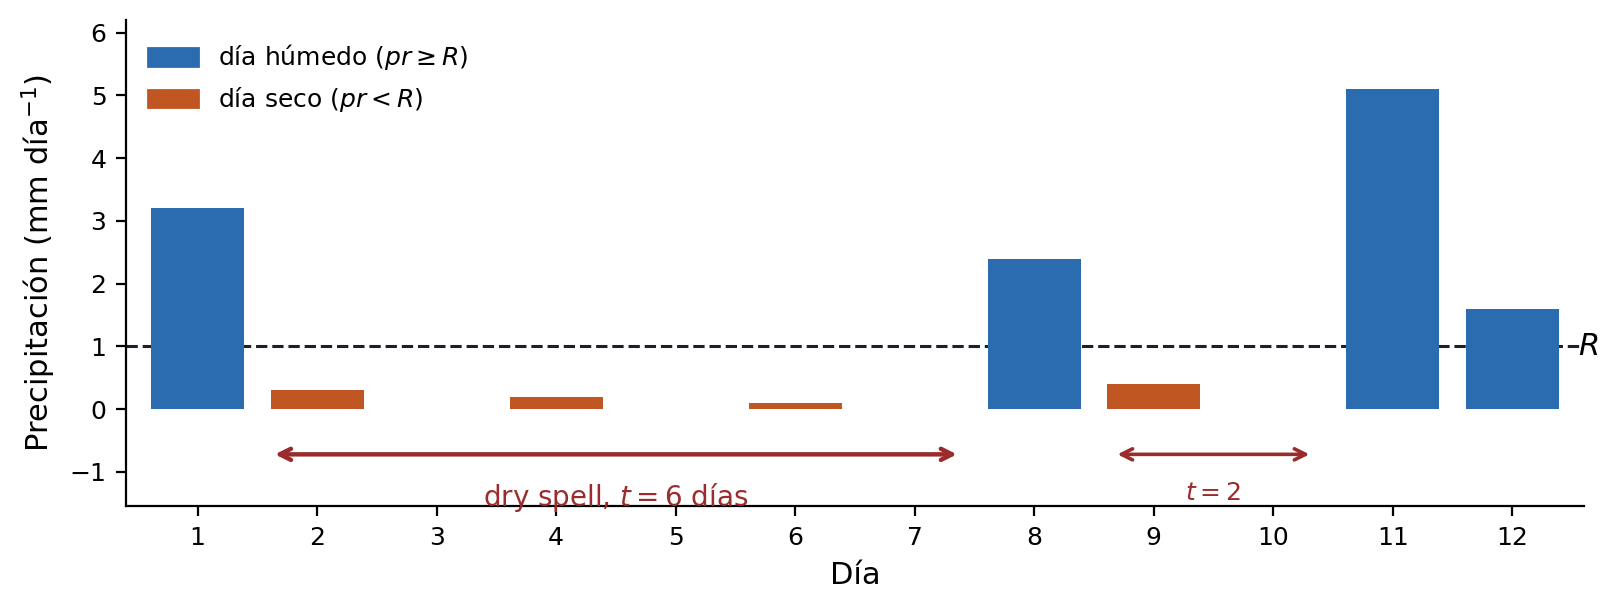
\includegraphics[width=1\linewidth,height=0.72\textheight,keepaspectratio,alt={Definición operativa. Un día es húmedo si pr ≥ R y seco si pr \textless{} R. Un dry spell es la racha consecutiva de días secos; su duración t es el número de días de la racha. En el ejemplo, R = 1 mm día$^{-1}$ produce un spell de t = 6 días y otro de t = 2 días, separados por un día húmedo. Los puntos marcan días secos con 0 mm.}]{fig_esquema_dryspell.png}
\caption[Definición operativa de día húmedo, día seco y dry spell]{Definición operativa. Un día es húmedo si pr ≥ R y seco si pr \textless{} R. Un dry spell es la racha consecutiva de días secos; su duración t es el número de días de la racha. En el ejemplo, R = 1 mm día$^{-1}$ produce un spell de t = 6 días y otro de t = 2 días, separados por un día húmedo. Los puntos marcan días secos con 0 mm.}\label{fig:esquema}
\end{figure}

La comparación histórica entre CR2MET y ALADIN requiere considerar sus diferencias en la frecuencia de días húmedos. Con R = 1 mm día$^{-1}$ en ambos productos, ALADIN presenta una fracción de días húmedos sustancialmente mayor que CR2MET (§\ref{sec:calibracion}), coherente con el sesgo de llovizna de los modelos (Stephens et al., 2010; Petrova et al., 2024; Martinez-Villalobos et al., 2022). Ese exceso fragmenta las rachas secas y produce spells artificialmente más cortos y numerosos, de modo que un umbral común de 1 mm no permite una comparación equitativa de la persistencia seca.

Por ello el análisis principal adopta el criterio i (umbral global calibrado): CR2MET con R = 1 mm día$^{-1}$ y ALADIN con R₀ = 5,285 mm día$^{-1}$, elegido para igualar la fracción espacial media de wet days de CR2MET a 1 mm (§\ref{sec:calibracion}). Este umbral dependiente del modelo sigue el criterio usado para evaluar PDFs de duración de dry spells frente a observaciones (Leung et al., 2022, sec.~3.b). Como sensibilidad se consideran el criterio ii (1 mm día$^{-1}$ en ambos) y el criterio iii (calibración local: un R₀(x,y) por píxel, de modo que en cada celda la fracción temporal de wet days de ALADIN iguale la de CR2MET a 1 mm). El criterio i es la configuración de los resultados principales; ii y iii permiten separar cuánto del sesgo histórico se debe a la definición de día húmedo y cuánto permanece como diferencia estructural del modelo (Tabla~\ref{tab:criterios}).

\begin{longtable}[]{@{}
  >{\raggedright\arraybackslash}p{(\linewidth - 6\tabcolsep) * \real{0.2500}}
  >{\raggedright\arraybackslash}p{(\linewidth - 6\tabcolsep) * \real{0.2500}}
  >{\raggedright\arraybackslash}p{(\linewidth - 6\tabcolsep) * \real{0.2500}}
  >{\raggedright\arraybackslash}p{(\linewidth - 6\tabcolsep) * \real{0.2500}}@{}}
\caption[Criterios de umbral para definir días húmedos]{Criterios de umbral para definir días húmedos. El análisis principal usa el criterio i.}\label{tab:criterios}\tabularnewline
\toprule\noalign{}
\begin{minipage}[b]{\linewidth}\raggedright
Criterio
\end{minipage} & \begin{minipage}[b]{\linewidth}\raggedright
CR2MET
\end{minipage} & \begin{minipage}[b]{\linewidth}\raggedright
ALADIN
\end{minipage} & \begin{minipage}[b]{\linewidth}\raggedright
Uso
\end{minipage} \\
\midrule\noalign{}
\endfirsthead
\toprule\noalign{}
\begin{minipage}[b]{\linewidth}\raggedright
Criterio
\end{minipage} & \begin{minipage}[b]{\linewidth}\raggedright
CR2MET
\end{minipage} & \begin{minipage}[b]{\linewidth}\raggedright
ALADIN
\end{minipage} & \begin{minipage}[b]{\linewidth}\raggedright
Uso
\end{minipage} \\
\midrule\noalign{}
\endhead
\bottomrule\noalign{}
\endlastfoot
i (global) & 1 mm & R₀ = 5,285 mm (único, Chile) & Resultados principales \\
ii (mismo umbral) & 1 mm & 1 mm & Sensibilidad: sesgo sin calibrar \\
iii (local) & 1 mm & R₀(x,y) por píxel & Sensibilidad espacial \\
\end{longtable}

\section{Calibración del umbral R₀}\label{sec:calibracion}

La calibración de R₀ busca el umbral tal que el promedio espacial sobre Chile continental de la fracción temporal de días con pr ≥ R en ALADIN iguale la fracción correspondiente de CR2MET con R = 1 mm día$^{-1}$. Si F(R) denota esa fracción espacial media de wet days, calculada con igual peso para cada celda de la grilla de ALADIN, se resuelve F\_ALADIN(R₀) = F\_CR2MET(1 mm) mediante bisección. En 1980--2014, CR2MET a 1 mm produce F = 20,94 \% y ALADIN a 1 mm produce F = 30,68 \% (+9,7 puntos porcentuales). El umbral R₀ = 5,285 mm día$^{-1}$ reproduce F = 20,94 \% en ALADIN (Figura~\ref{fig:calibracion}).

\begin{figure}[htbp]
\centering
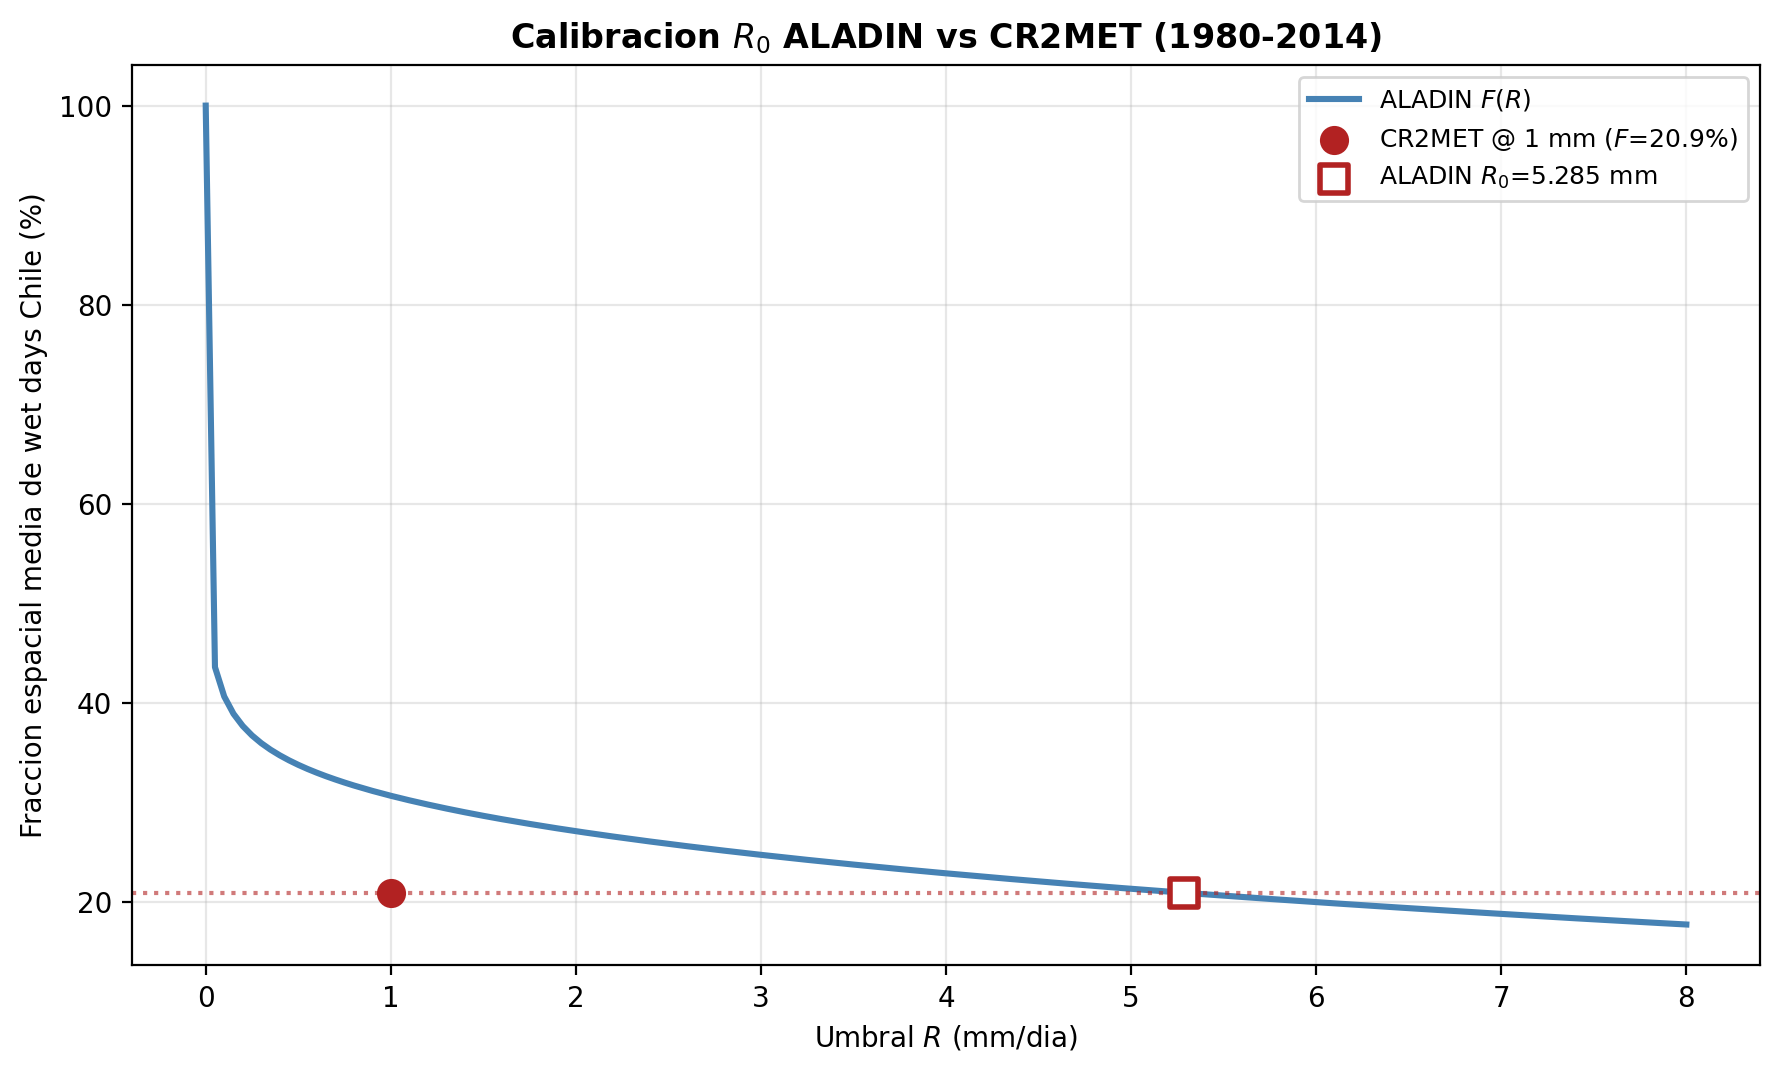
\includegraphics[width=1\linewidth,height=0.72\textheight,keepaspectratio,alt={Calibración del umbral de día húmedo en ALADIN frente a CR2MET (1980--2014). La curva azul es F(R), la fracción media de días húmedos de ALADIN en Chile continental en función del umbral R. El punto azul es ALADIN a 1 mm (F = 30,7 \%) y el punto rojo es CR2MET a 1 mm (F = 20,9 \%); la flecha indica el exceso de días húmedos de ALADIN (+9,7 puntos porcentuales), que, sin calibrar, acorta las rachas secas. El cuadrado marca R₀ = 5,285 mm día$^{-1}$, umbral con el que ALADIN iguala la fracción de CR2MET.}]{fig03_calibracion_R0_ftau.png}
\caption[Calibración del umbral de día húmedo en ALADIN frente a CR2MET (1980--2014)]{Calibración del umbral de día húmedo en ALADIN frente a CR2MET (1980--2014). La curva azul es F(R), la fracción media de días húmedos de ALADIN en Chile continental en función del umbral R. El punto azul es ALADIN a 1 mm (F = 30,7 \%) y el punto rojo es CR2MET a 1 mm (F = 20,9 \%); la flecha indica el exceso de días húmedos de ALADIN (+9,7 puntos porcentuales), que, sin calibrar, acorta las rachas secas. El cuadrado marca R₀ = 5,285 mm día$^{-1}$, umbral con el que ALADIN iguala la fracción de CR2MET.}\label{fig:calibracion}
\end{figure}

R₀ representa un umbral que hace equivalentes las frecuencias de días húmedos de ambos productos: un día de ALADIN con 3 mm se trata como seco porque, en frecuencia, corresponde a un día bajo 1 mm en CR2MET. La calibración iguala la frecuencia en promedio sobre Chile, no en cada celda; el criterio iii (§\ref{sec:definicion}) evalúa ese efecto calibrando un umbral por píxel. Igualar la frecuencia de días húmedos tampoco impone que se distribuyan igual en el tiempo: dos series con el mismo número de días húmedos pueden producir rachas secas muy distintas si esos días aparecen agrupados o dispersos. Por ello, las diferencias de duración que persisten tras la calibración reflejan la organización temporal de la precipitación en el modelo y no solo su exceso de días húmedos.

\section{Construcción y normalización de las PDFs}\label{sec:pdfs}

Para caracterizar la distribución de duraciones se construyen PDFs empíricas de la variable t (días), con bins uniformes en log₁₀(t), siguiendo la convención de PDFs de precipitación diaria (Martinez-Villalobos y Neelin, 2018; Martinez-Villalobos et al., 2022). En cada cuenca se usan los mismos bins para CR2MET, ALADIN histórico y ALADIN futuro: se generan 26 bordes en escala logarítmica entre 1 día y la duración máxima observada entre los tres conjuntos, y se redondean a enteros. Como las duraciones son enteras, los bordes repetidos se fusionan, de modo que cada bin contiene un número entero de días y el número efectivo de bins es de 21 a 23 según la cuenca.

En cada bin, f(t) es el número de spells en el intervalo dividido por el ancho de bin, de modo que el área bajo la curva es igual al número total de spells del pool y los cambios en frecuencias y en forma son visibles a la vez. El binning solo afecta la representación gráfica: los estadísticos de la Tabla~\ref{tab:estadisticos} y los risk ratios se calculan directamente sobre las duraciones.

\section{Agrupación regional y estadísticas espaciales}\label{sec:pool}

Para las PDFs por cuenca se adopta un pool regional: todos los dry spells de todos los píxeles de la ventana se agrupan en un único conjunto de eventos (Martinez-Villalobos y Neelin, 2018). El pool aumenta el tamaño muestral y permite resolver la cola; a cambio, mezcla heterogeneidad espacial dentro de la caja. Como los píxeles vecinos no son independientes, n\_spells no debe leerse como tamaño muestral efectivo para inferencia estadística.

Para los mapas se calculan, en cada píxel, la duración media y el percentil 99 de las duraciones (t99), y se reportan las diferencias Δ = ALADIN − CR2MET en 1980--2014. Los estadísticos solo se calculan en píxeles con al menos 30 spells en el período. La significancia de Δ se evalúa con bootstrap por años (1 000 réplicas). Primero se identifican los spells en la serie diaria de cada píxel con las reglas de §\ref{sec:definicion}, incluida la exclusión de rachas censuradas en los bordes del período. Cada spell conserva su duración íntegra aunque cruce el 1 de enero y se asigna al año calendario de su inicio. Con ello se forma, por píxel y producto, un conjunto \{año: vector de duraciones\}.

En cada réplica se sortean 35 años calendario con reemplazo, usando el mismo sorteo para CR2MET y ALADIN (bootstrap pareado). Se concatenan las duraciones de todos los spells cuyo año de inicio figura en el sorteo y se recalculan la media o t99 de cada producto y su diferencia Δ\emph{. El intervalo de confianza al 95 \% de Δ corresponde a los percentiles 2,5 y 97,5 de las 1 000 réplicas de Δ}, y Δ se considera significativo cuando el intervalo no incluye el cero.

Como se evalúan unas 3 500 celdas con α = 5 \%, cabe esperar que alrededor del 5 \% resulte significativo por azar; los porcentajes de celdas significativas se interpretan en relación con esa referencia.

\section{Risk ratios y cambios futuros}\label{sec:rr}

El cambio proyectado en la ocurrencia de dry spells largos se cuantifica con el risk ratio

\emph{(1) RR(D) = N\_fut(t ≥ D) / N\_hist(t ≥ D)}

donde N(t ≥ D) es el número de dry spells con duración de al menos D días en ALADIN futuro (2040--2074) e histórico (1980--2014), ambos con R₀ = 5,285 mm día$^{-1}$ y con las reglas de §\ref{sec:definicion}, incluida la exclusión de rachas censuradas. Como ambos períodos tienen la misma longitud (35 años), RR(D) es también una razón de frecuencias; RR(D) \textgreater{} 1 indica más rachas largas en el futuro. Al no normalizar por el número total de spells de cada período, RR(D) es consistente con las PDFs (§\ref{sec:pdfs}) y refleja el cambio en la ocurrencia de eventos largos, no solo en su fracción relativa.

Los risk ratios se calculan sobre pools de las cuatro regiones administrativas (§\ref{sec:datos}), considerando solo spells cuyo día de inicio cae entre marzo y noviembre (otoño, invierno y primavera), meses que concentran entre el 85 \% y el 97 \% de la precipitación anual en esas regiones. En verano la precipitación es escasa, sobre todo en Chile central, y las rachas largas forman parte del ciclo estacional esperado; los spells que comienzan en noviembre se cuentan con su duración completa aunque se extiendan al verano. Las PDFs, en cambio, incluyen spells de todo el año. Se calculan curvas RR(D) para D entre 5 y 60 días, y D = 20 días se usa como valor de referencia porque corresponde aproximadamente al percentil 90 de las duraciones en Chile central (Tabla~\ref{tab:estadisticos}). Los intervalos de confianza al 95 \% se obtienen con bootstrap por años (1 000 réplicas): en cada réplica se sortean con reemplazo 35 años de inicio del histórico y, de forma independiente, 35 del futuro, y se recalcula el cociente de conteos. Como se remuestrean años completos para todos los píxeles de la región a la vez, el procedimiento conserva la correlación espacial entre píxeles. El cambio se considera significativo cuando el IC95 queda por completo por encima de 1 (aumento) o por debajo de 1 (disminución). Como la curva evalúa varios valores de D, se interpreta su comportamiento conjunto y no un umbral aislado.

\section{Sensibilidad a la elección del umbral}\label{sec:sensibilidad}

Para evaluar cuánto dependen los resultados de la definición de día húmedo, la comparación histórica entre CR2MET y ALADIN se repite con los tres criterios de la Tabla~\ref{tab:criterios}. A escala de Chile continental, se recalculan los mapas de duración media y t99, sus diferencias Δ y su significancia con el procedimiento de §\ref{sec:pool}. A escala de cuenca, se comparan las PDFs de Loa, Maipo, Maule y Biobío en 1980--2014 para CR2MET a 1 mm y para ALADIN a 1 mm, a R₀ global y a R₀ local, con los bins de §\ref{sec:pdfs}. Además, los risk ratios de §\ref{sec:rr} se recalculan con 1 mm en ALADIN para comprobar que la señal futura no depende de la calibración. Los resultados de estas pruebas (Tablas~\ref{tab:S1}--\ref{tab:S3}, Figuras~\ref{fig:S1} y~\ref{fig:S3}) y el mapa de R₀ local (Figura~\ref{fig:S2}) se presentan en el material suplementario.

\section{Herramientas computacionales y reproducibilidad}\label{sec:software}

\pendiente{describir el software (Python, xarray, numpy, cartopy) y remitir al
Anexo B con los scripts que generan cada figura y tabla.}

\pendiente{agregar un diagrama de flujo de la metodología: datos → regrillado →
definición de rachas → calibración de R₀ → PDFs, mapas y bootstrap →
risk ratios → sensibilidades.}
